\section{2D-Repräsenation}
\setauthor{Felix Dumfarth}

\subsection{Frontend}
Der Chatbot der HTL Leonding sollte auf der Schulhompage als Chatblase angezeigt werden, und verschiedene Elemente wie Buttons und Links unterstzützen.
\subsubsection{Konzept}
Während den Anfängen der Diplomarbeit wurde ein Konzept erstellt, um das mögliche Aussehen festzulegen. Lange Zeit wurde der Chatbot unter den Namen Leon geführt. 
Dies wurde jedoch im späteren verlauf geändert und Leon wurde Teil des langjährigen Leonie Projektes der HTL Leonding.
Ursprünglich war das Symbol des Chatbots, wie man am Konzept sehen kann, ein Bot. Durch den wechsel in die Leonie Familie wurde dieses Logo jedoch gegen Leonie getauscht.
\begin{figure}[hbt!]
    \centering
    \includegraphics[scale=0.2]{pics/conceptBotClosed.png}
    \caption{Konzept Chatbot geschlossen}
    \label{fig:impl:conceptBotClosed}
\end{figure}
\begin{figure}[hbt!]
    \centering
    \includegraphics[scale=0.2]{pics/conceptBotOpen.png}
    \caption{Konzept Chatbot geöffnet}
    \label{fig:impl:conceptBotOpen}
\end{figure}

\subsubsection{Umsetzung}
Umgesetzt wurde das Frontend mitthilfe von Angular. Die Chatblase ist eine eigene Komponente, die durch CSS immer rechts unten fixiert ist. Die Farben des Chatbots sollten natürlich an die HTL Leonding erinnern, deshalb wurde ein Farbverlauf aus Farben des HTL Logos erstellt.

Jedoch begann der Chatbot sehr anders, zu beginn wurde der Bot zuerst als ganze Seite entwickelt und nicht nur als Chatblase.
\begin{figure}[hbt!]
    \centering
    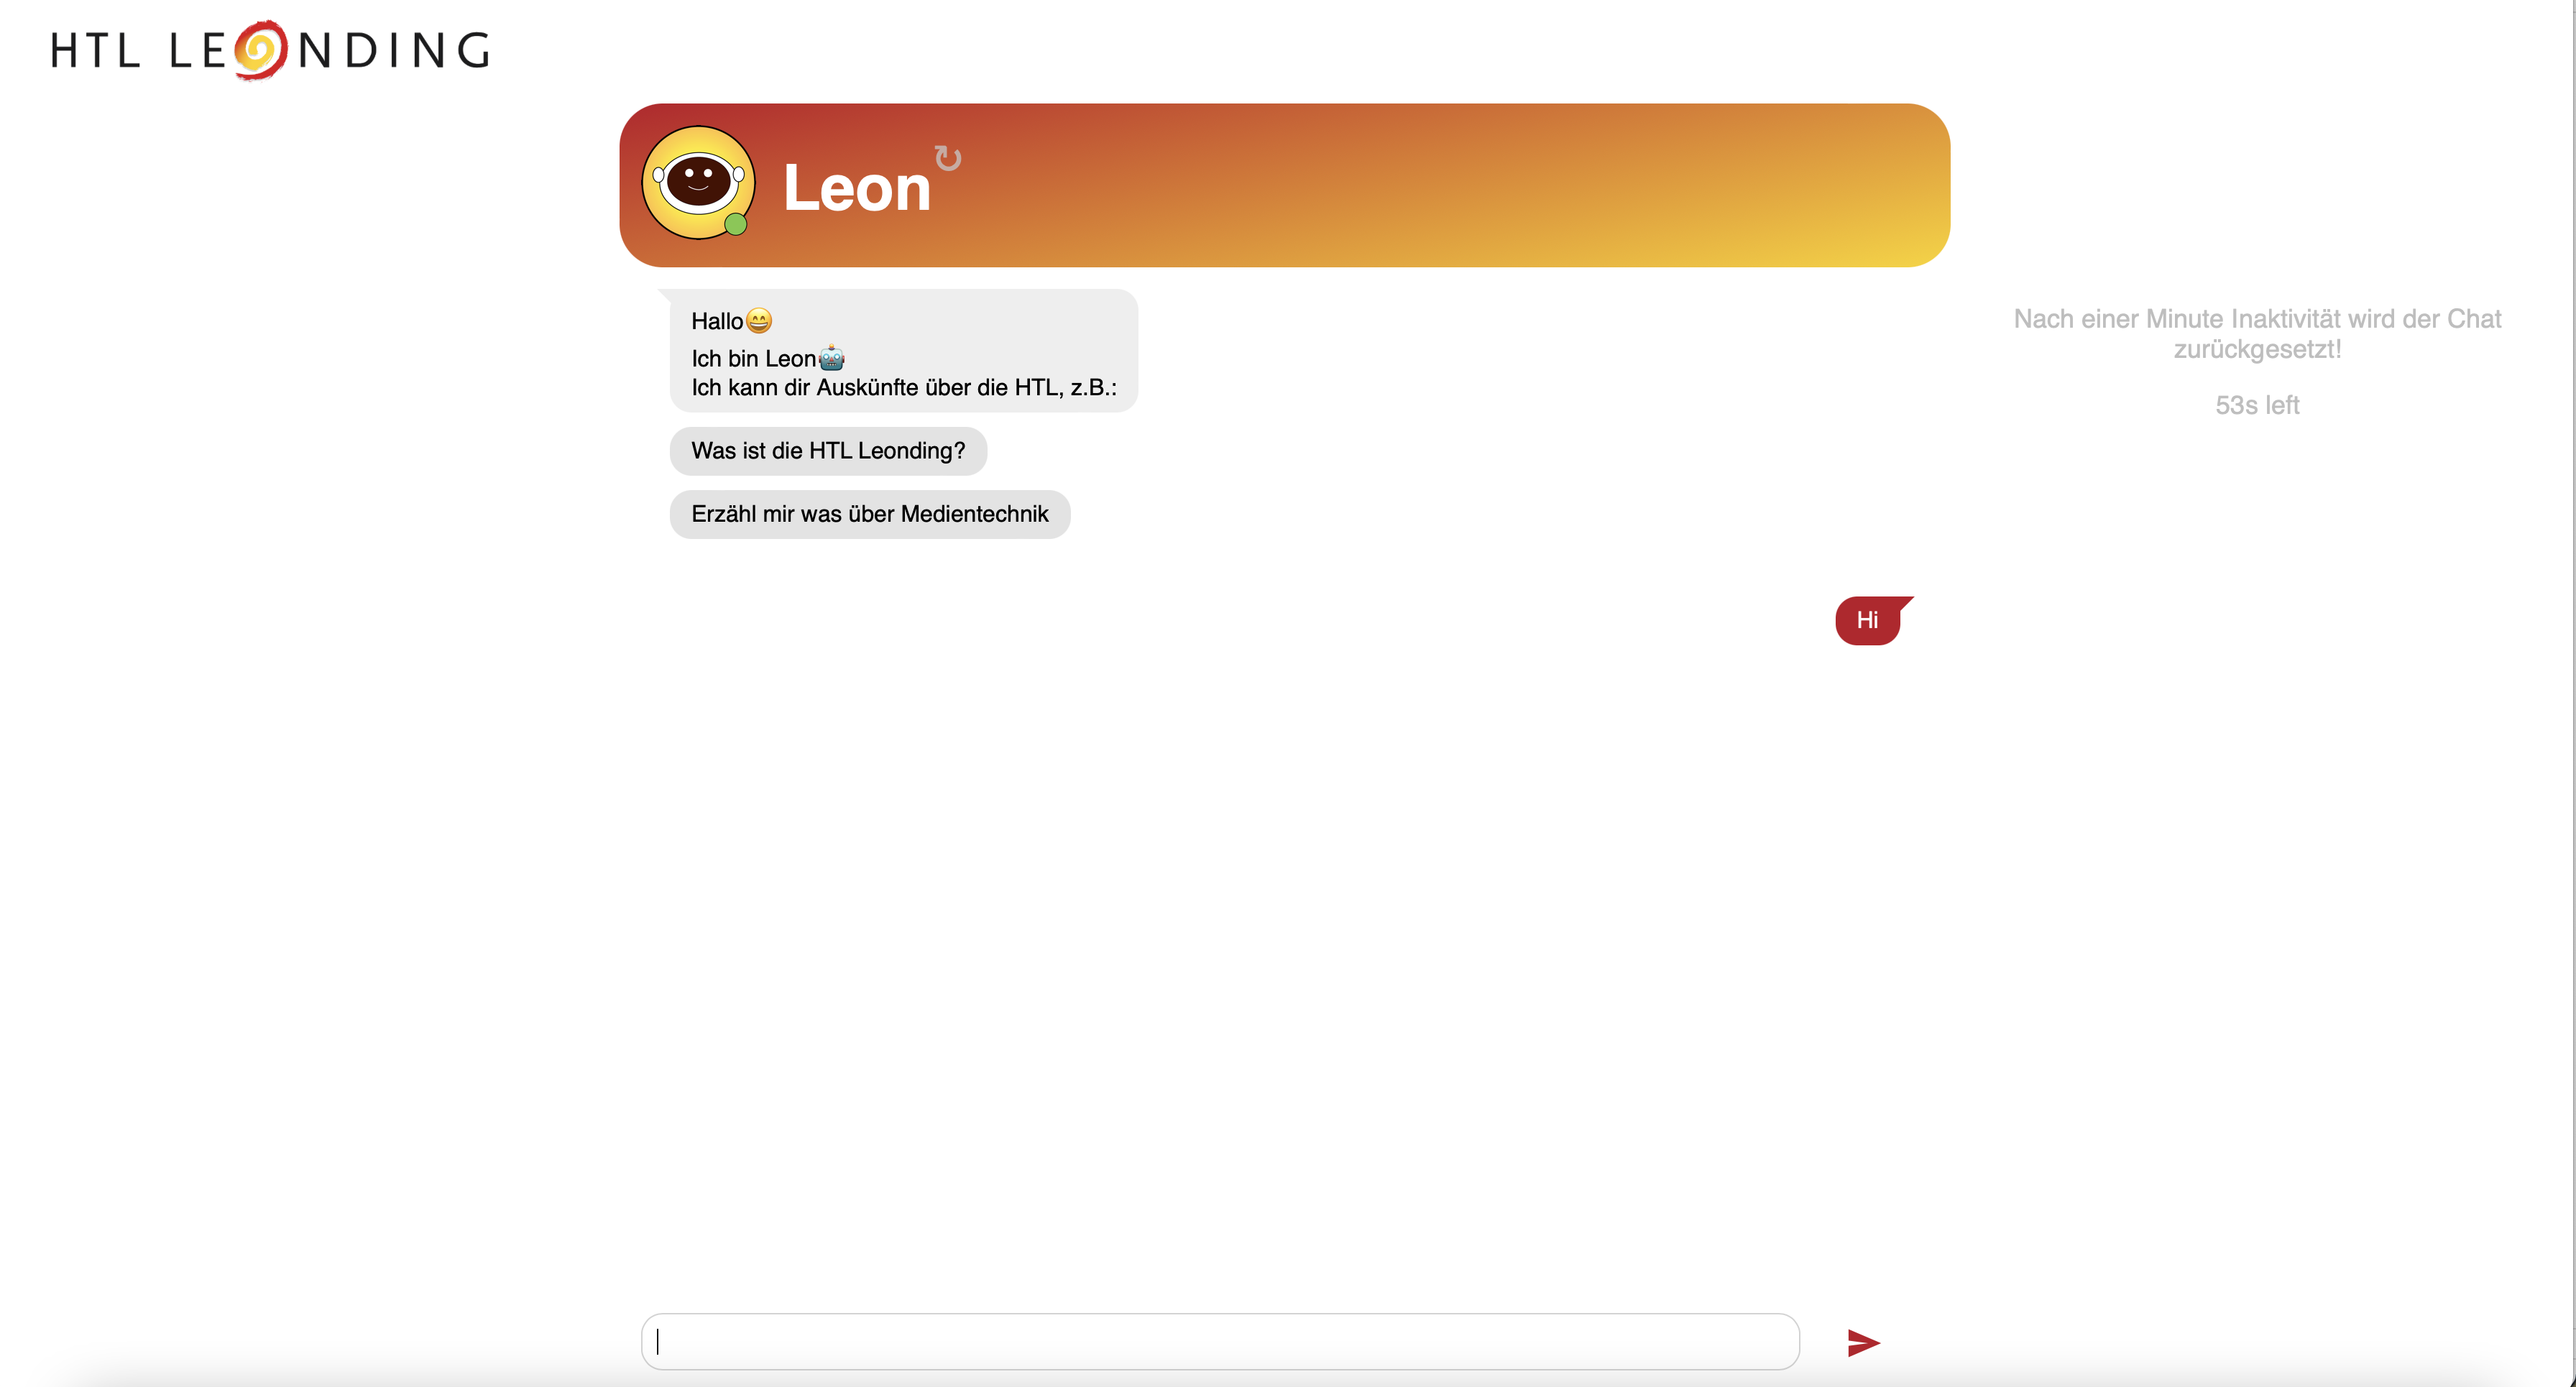
\includegraphics[scale=0.2]{pics/fullPageBot.png}
    \caption{Chatbot auf einer ganzen Seite}
    \label{fig:impl:conceptBotFullPage}
\end{figure}

Natürlich war dies nicht das entgültige Ziel so wurde der Bot schnell zur Chatblase umgewandelt.
Zum testen war die HTL Leonding Seite mithilfe eines IFrames eingebunden und zusätzlich Chatblase.

Um das Gespräch in eine Richtung zu lenken wurden Buttons eingeführt, die nach fast jeder Antwort mögliche folge Fragen vorschlagen.

\begin{figure}[hbt!]
    \centering
    \includegraphics[scale=0.2]{pics/finalBot.png}
    \caption{Chatbot}
    \label{fig:impl:bot}
\end{figure}

Um Bewertungen von echten Benutzern zu holen wurde außerdem eine Feedback Seite eingeführt, in dieser kann der Benutzer eine 1 bis 5 Sterne bewertung und einen Text absenden.


\subsection{Dashboard}

Um alle Gespräche und die Bewertungen der Benutzer anzuzeigen wurde ein Dashboard eingeführt, wo nur dies möglich war.
Im Laufe der Diplomarbeit wurde dieses dann erweitert, um für den Leobot Conversation Cycle als Seite zu dienen.

Einerseits kann man sich die vergangenen Unterhaltungen ansehen, so wie die nlu.yml, stories.yml, rules.yml, domain.yml direkt im Monaco Editor bearbeiten und speichern.

\begin{figure}[hbt!]
    \centering
    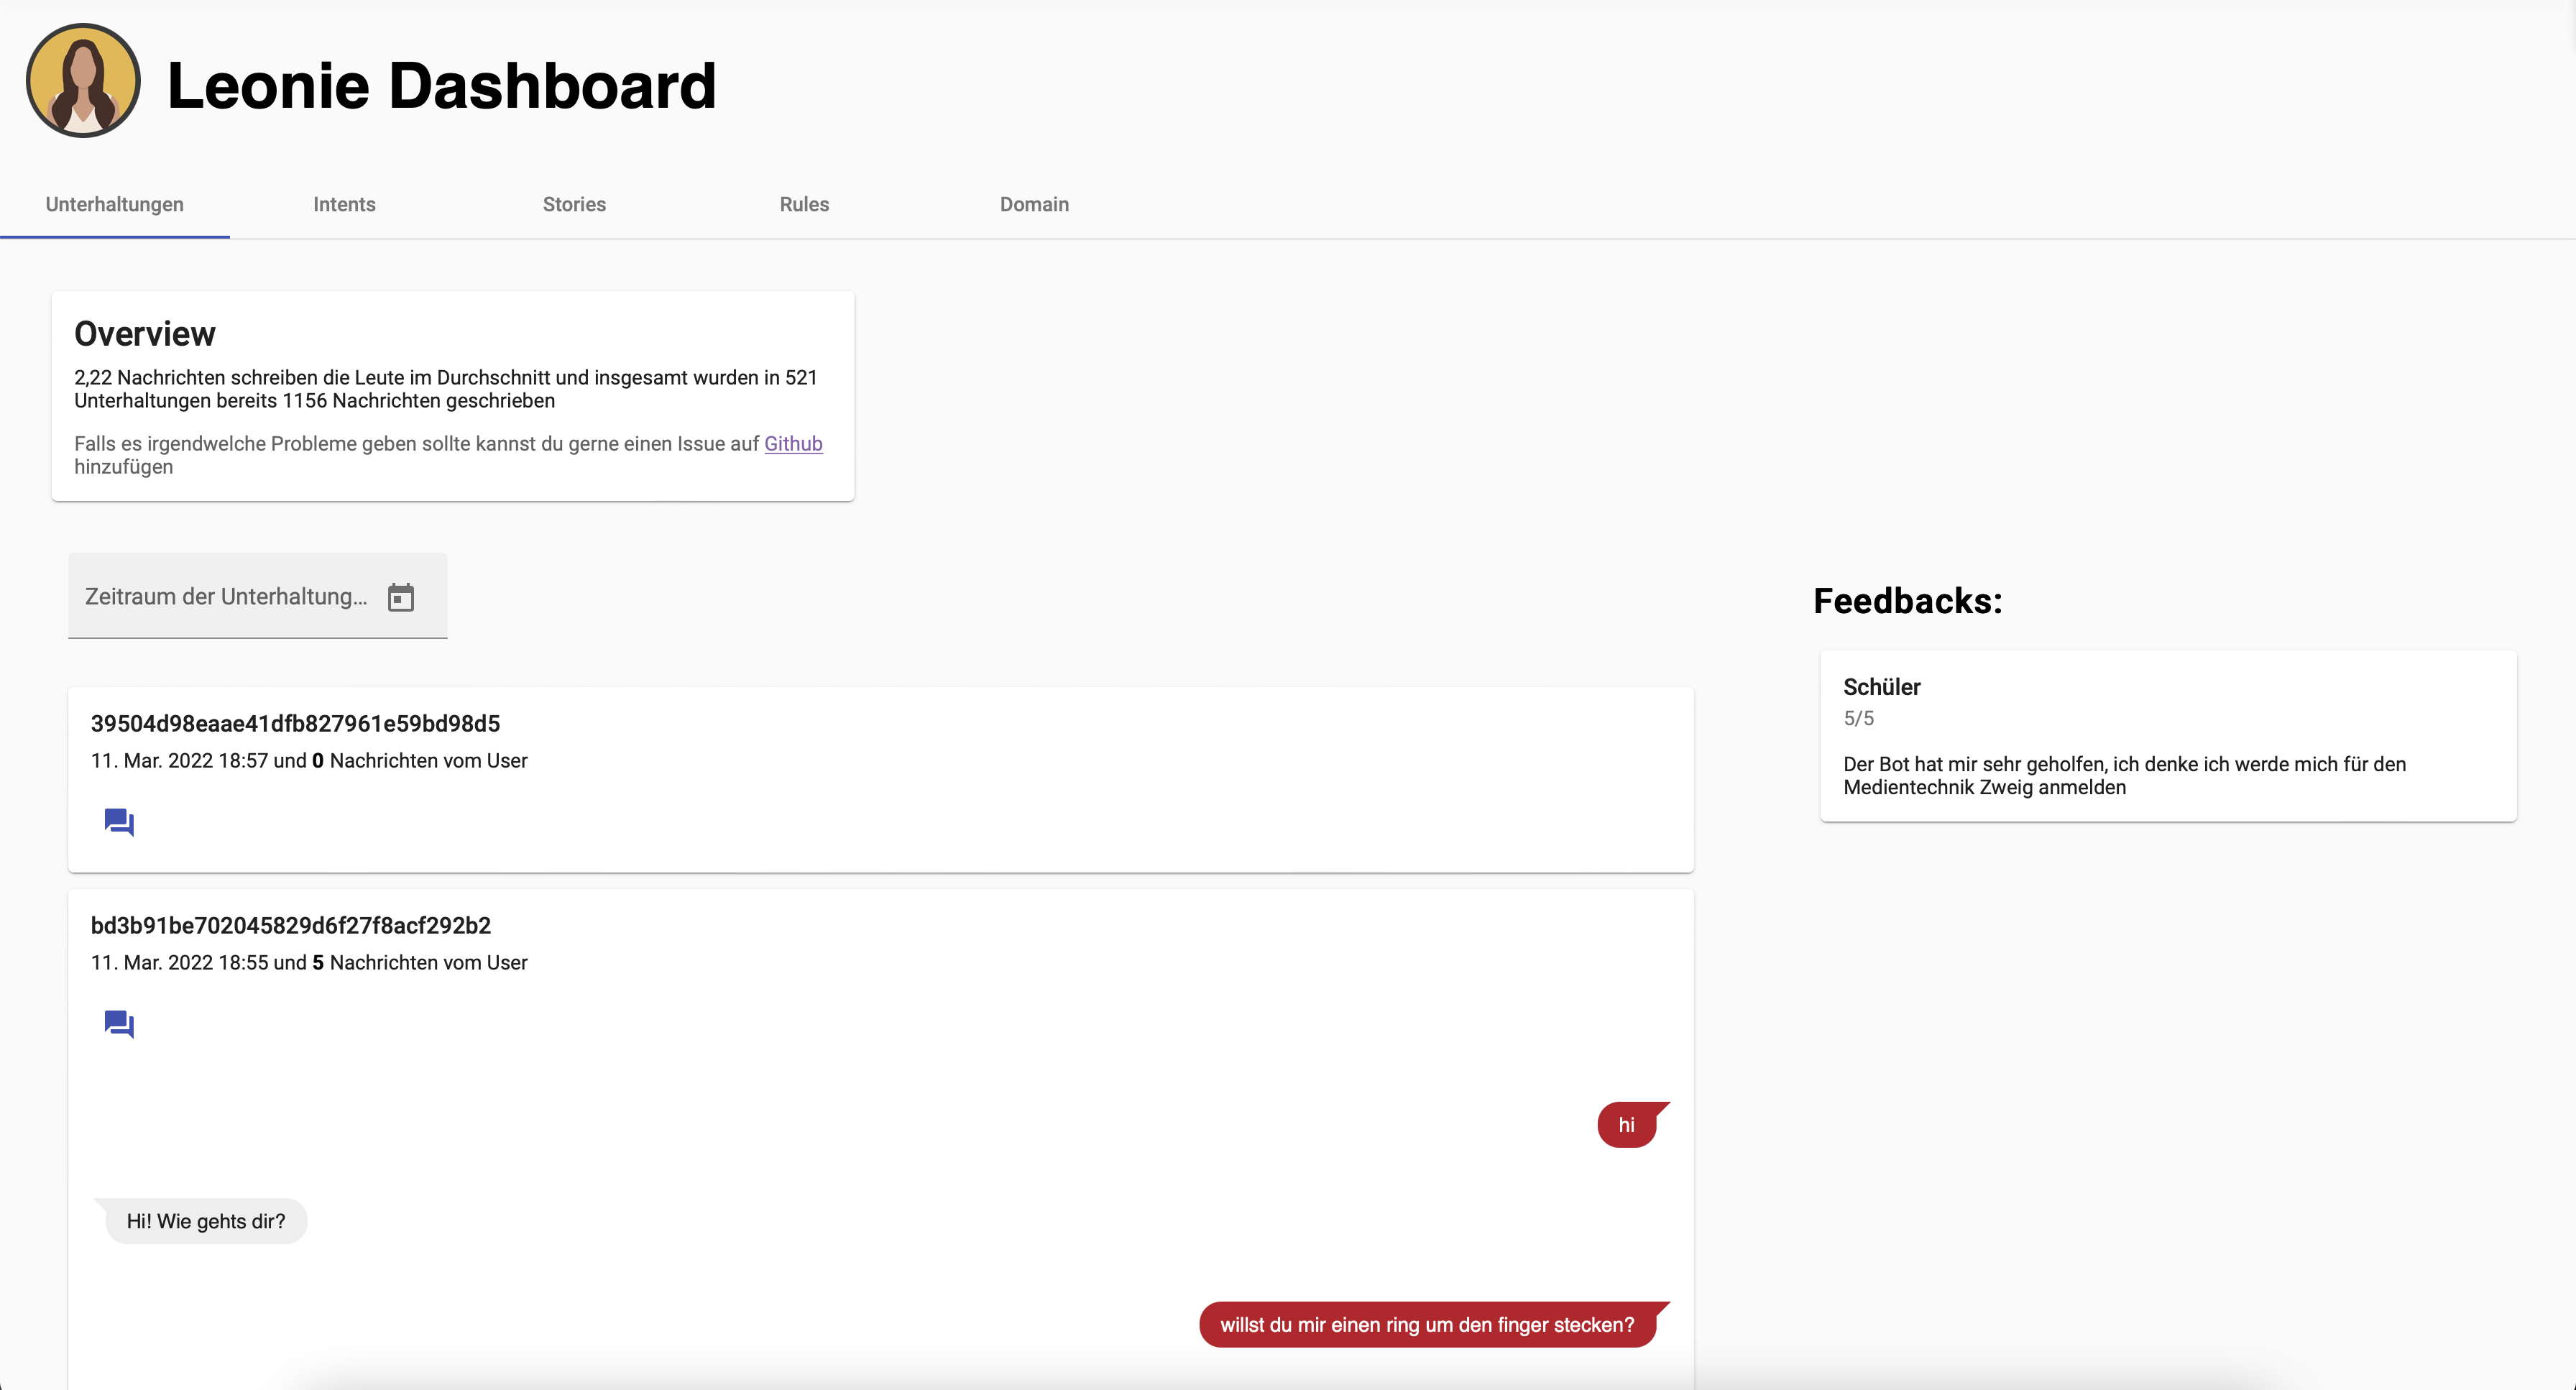
\includegraphics[scale=0.2]{pics/dashboardConvo}
    \caption{Dashboard}
    \label{fig:impl:dashConv}
\end{figure}

Im Editor wurden auch Code Vorschläge benutzt um etwas an Tipparbeit sparen zu können.

\begin{figure}[hbt!]
    \centering
    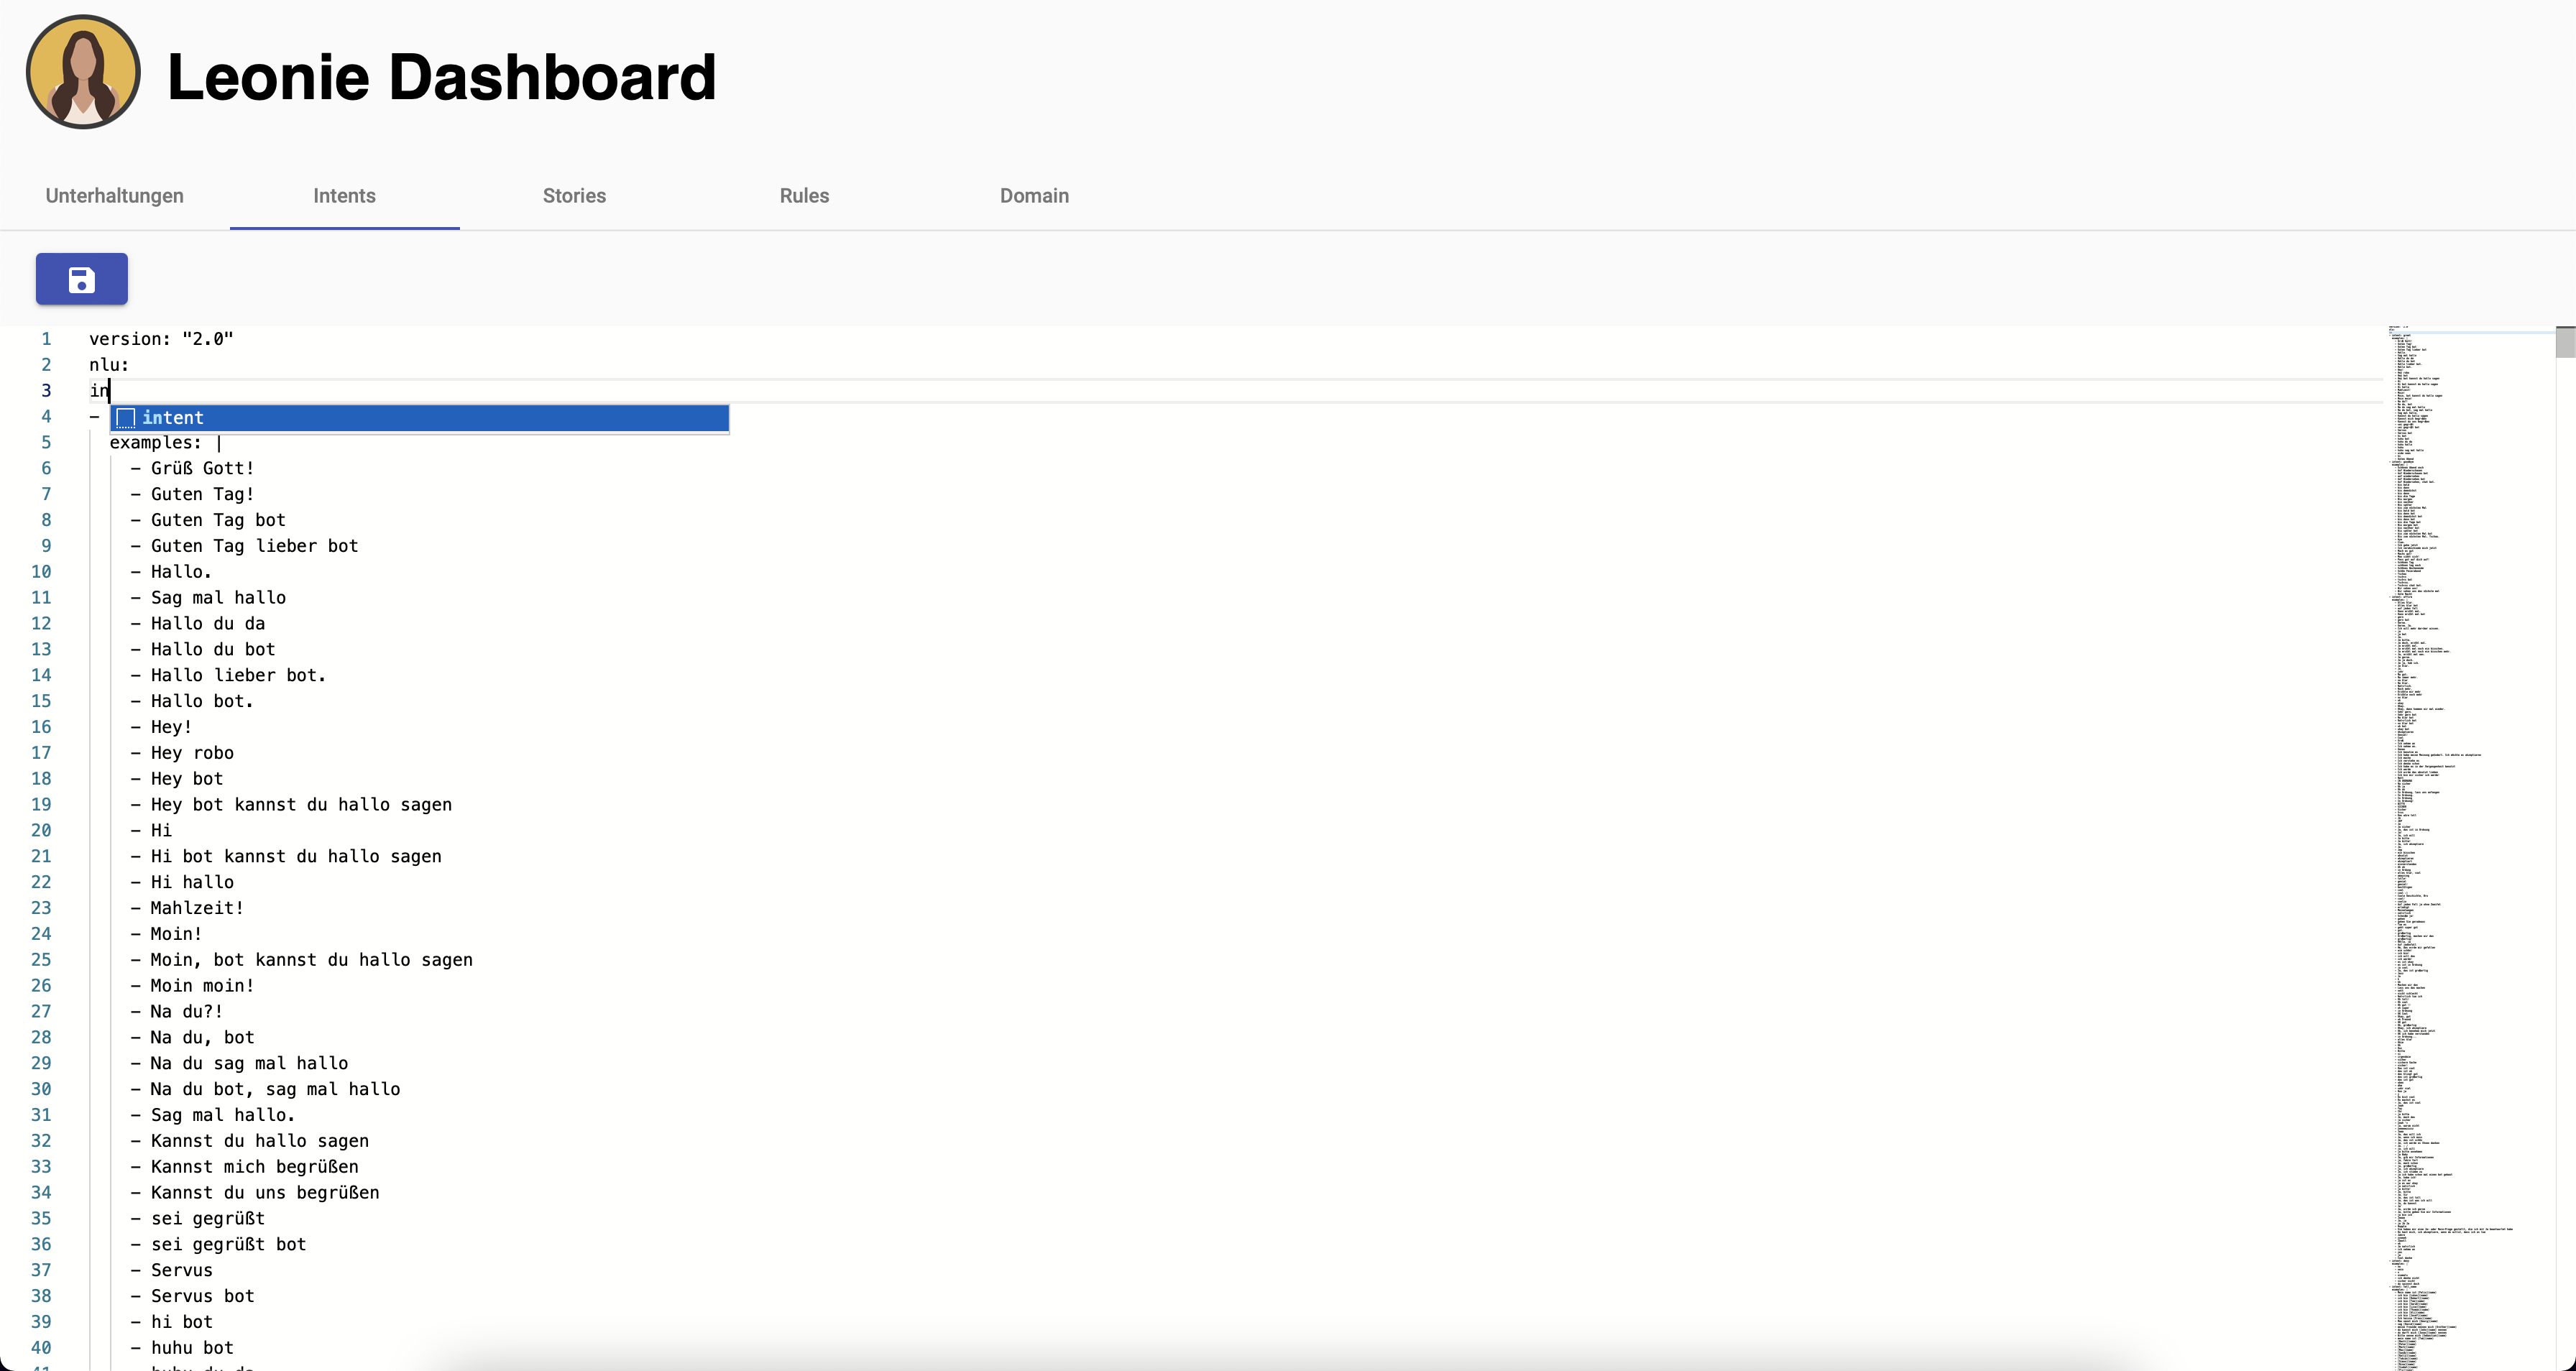
\includegraphics[scale=0.2]{pics/dashboardCodeSuggestion}
    \caption{Vorschläge}
    \label{fig:impl:dashboardCodeSuggestion}
\end{figure}
\begin{figure}[hbt!]
    \centering
    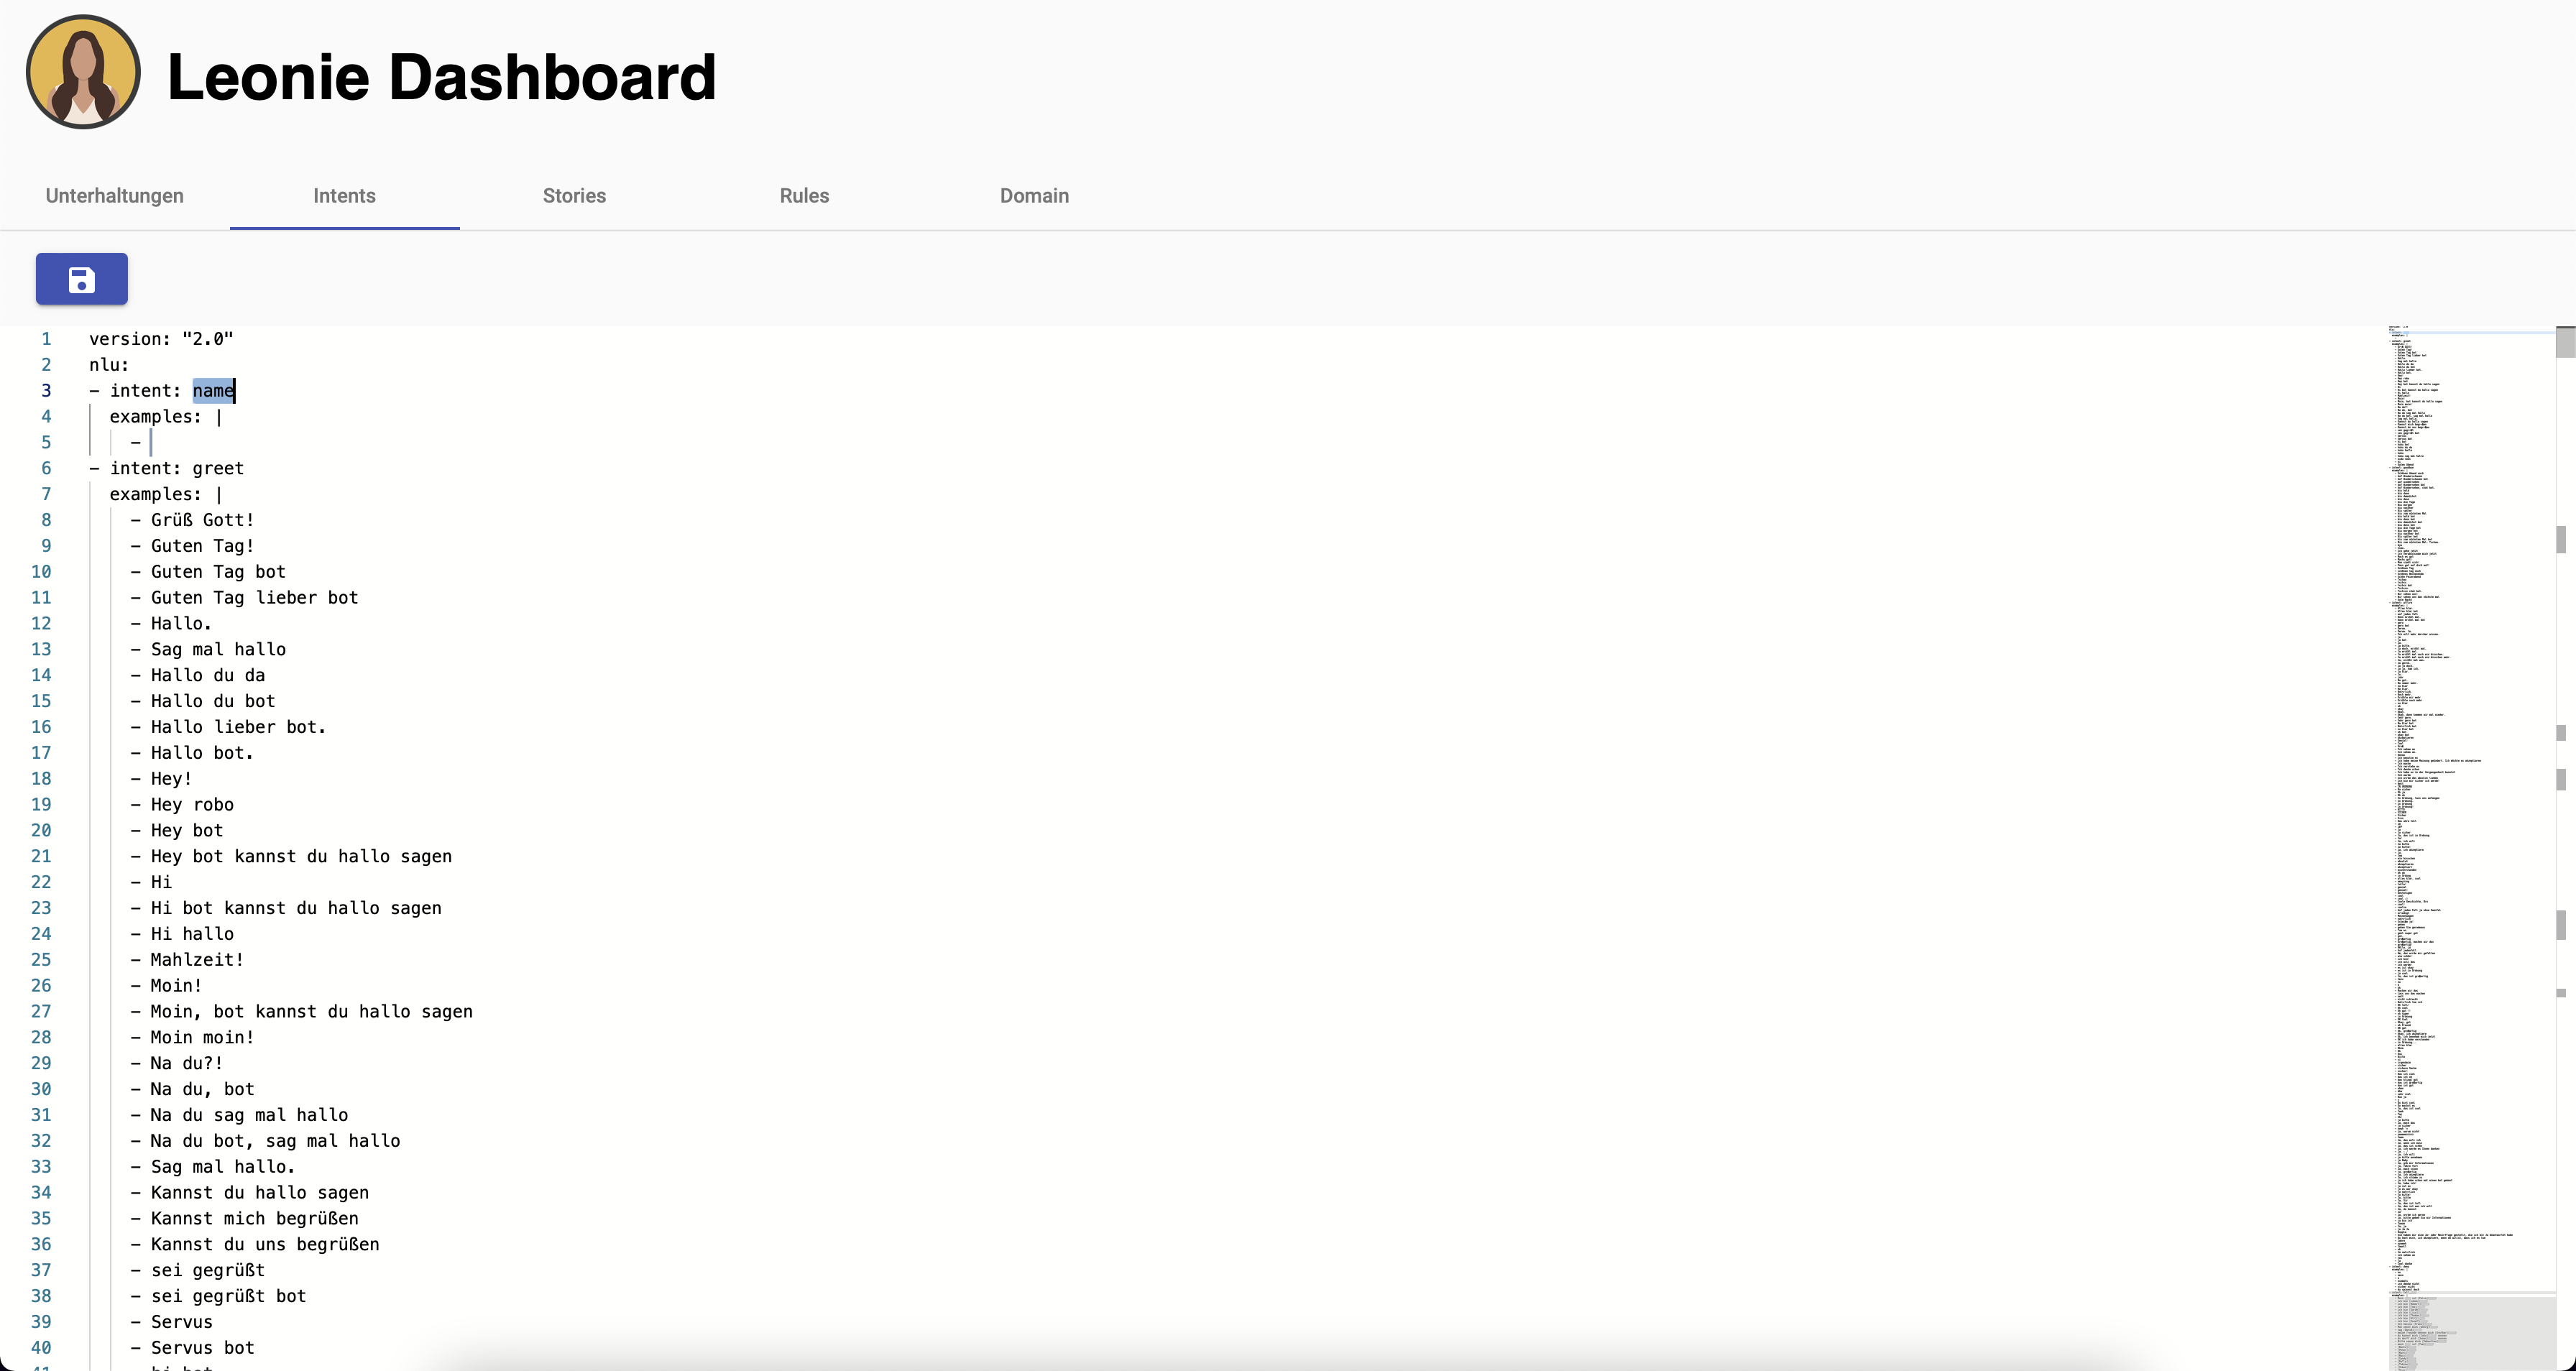
\includegraphics[scale=0.2]{pics/dashboardSuggestionMade}
    \caption{Vorschlag benutzt}
    \label{fig:impl:dashboardCodeSuggestionMade}
\end{figure}



\subsection{Einbindung in Wordpress}
\subsubsection{Angular Elements}
''Webkomponenten sind eine Gruppe von Web-Technologien, die es ermöglichen, benutzerdefinierte, wiederverwendbare HTML Elemente zu erstellen, deren Funktionalität gekapselt ist und damit vollständig getrennt von anderem Code.''\cite{webcomponents}


\section{Schwierigkeiten}
\setauthor{Felix Dumfarth}
